\chapter{Literature Review}
\section{Thermocouple Array}
Few studies have proposed methods for continuous monitoring of the snowpack temperature profile. One successful instrument is the SM4 snowpack temperature and snow depth sensor. The NIVEXC is another instrument that has been used to record temperature profile measurements. Both of these systems are installed at avalanche starting zones and they measure temperature gradients using thermistors. In addition to these sensors designed for avalanche starting areas, \cite{conway_benedict_1994} created a thermistor array designed to study the infiltration of water during rain-on-snow events. 

\subsection{\cite{ingolfsson2008sm4}}  The main objective of the SM4 is to accurately measure snow depth in avalanche starting areas. The SM4 is series of digital thermistors mounted with a fixed 20cm interval on a pole that extends through the snowpack (Fig. \ref{fig:SM4}). The SM4 Measures snow depth by identifying thermistors buried in the snow, based on damping of temperature fluctuations that is caused by the snowpack. (\cite{ingolfsson2008sm4}) have developed an algorithm that calculates the snow depth as a function of the temperature profile. This snow depth algorithm is proving to be more reliable than acoustic snow depth sensors because it functions during times of snowfall and ice buildup. The main challenge regarding the algorithm is greatest when the temperature of the atmosphere approaches the temperature of the snowpack. It is typically installed in avalanche starting areas where it is coupled with ultrasonic snow depth sensors for verification. Measurements are logged with a few minute interval and are regularly transferred to a central computer through wireless GSM telephone connection.

In addition to snow depth, the SM4 is being used to detect and visualize high temperature gradients within the snowpack. The critical gradient assumed to produce facets in the snowpack is 0.1\textdegree C/cm \cite{mcclung_schaerer_2009}. Each time the temperature profile between two thermistors exceeds this critical gradient, a red dot is marked on a continuous snow depth plot. When this temperature gradient continues for some time period, it appears as a red line which indicates an area of potential facet formation. 

 \begin{figure}[!t]
    \centering
    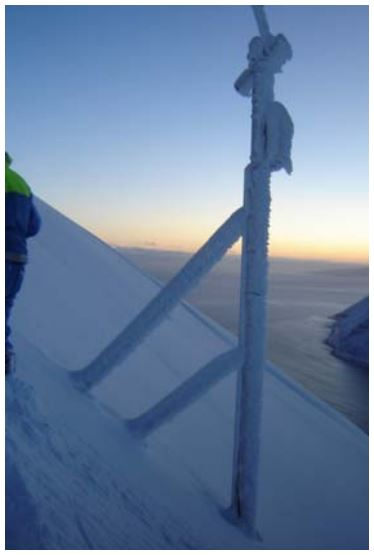
\includegraphics[width=0.8\linewidth]{figures/SM4.JPG}
    \caption{An ultrasonic sensor and a SM4 snow depth sensor covered with icing. The SM4 is attached to the upper stanchion.}
    \label{fig:SM4}
 \end{figure}
 
\subsection{\cite{barbolininivexc}}  
Like the SM4, the NIVEXC is designed to accurately measure snow depth in avalanche starting areas. The NIVEXC is an electronic snow-pole with a vertical array of sensors. NIVEXC is able to record and transmit important snow cover properties, such as total snow height, snow precipitation amounts and rates, and temperature profiles. The pole is equipped with 14 sensor boxes, mutually seperated by a 20 cm gap. Each sensor box includes three different types of sensors: (i) a pair of optical sensors (IR LED and photodiodes), functional to snow depth measurements, (ii) a temperature-dependent resistor (RTD), and (iii) a pair of electrodes, used to cross-validate snow depth data derived from optical sensors. Frequency of measurements and number of daily data transmissions can be set based on user needs, and can be remotely varied during operation. This particular sensor is currently installed in an avalanche release zone on a slope with north exposure and 35\textdegree inclination. NIVEXC optical sensors provide direct real-time information regarding snow depth. They observe that temperature fluctuations were greater for the sensors above the snow surface than for the ones buried in the snow. The depth at which temperature fluctuations become damped can be used for an indirect estimate of snow depth. However, the crater that sometimes forms around the pole can cause errors in the indirect estimate of total snow depth by temperature data. 

\subsection{\cite{conway_benedict_1994}} 
In \cite{conway_benedict_1994}, a rectangular grid of thermistors is used to study the infiltration of water during two midwinter rain on snow events. The progress of wetting is tracked in real time by monitoring changes in the position of the zero-degree isotherm. \cite{conway_benedict_1994} used these methods to calculate the infiltration rate and found that infiltration was not uniform. Water penetrated through localized channels that often occupied less than 50\% of the total volume of the snowpack. Their sensor was installed at 915m elevation in the Cascade Mountains near Snoqualmie Pass, Washington during 1991--1992. Measurements were made at 15-min intervals using up to 110 thermistors (Thermometrics p100DA202M) multiplexed to a data logger. The thermistors were wrapped in white heat-shrink tubing and white epoxy to make them waterproof and minimize heating from solar radiation. Each thermistor was field calibrated at the melting point for seasonal snow. Calibration was achieved at a time when the snow surrounding the thermistor was saturated and the electrical resistance of the thermistor had stabilized to a constant temperature. The temperature of saturated snow is likely to be slightly less than 0\textdegree C, but they assigned this temperature to 0\textdegree C. The temperature resolution was better than $\pm$ 0.01 \textdegree C.
 
The thermistors were arranged in a vertical, rectangular grid 1.5 m wide and up to 2 m deep. Each string consisted of 11 thermistors spaced 15 cm apart. A parallel horizontal string set at the same height 1 m away supported the leads from the thermistor beads to the multiplexer. The vertical spacing between thermistors was about 15 cm, but the thermistors were free to settle with the snowpack and the spacing decreased with time. 

\subsection{\cite{Black_Luce}}


\section{Stable Water Isotopes} 
Stable water isotopes can be used to better understand snow hydrological processes (\cite{beria_larsen_ceperley_michelon_vennemann_schaefli_2017}). The effect of different snow ablation processes (sublimation, melting, and redistribution) can be seen in the isotopic evolution of a seasonal snowpack (\cite{beria_larsen_ceperley_michelon_vennemann_schaefli_2017}). Water Isotopes represent a potential independent measure of sublimation in seasonal snow cover, although the majority of work in this area has focused on hydrograph separation (\cite{gustafson2010estimating}). Sommerfel (1987) and Gustafson (2010) found that isotope fractionation, driven by high vapor pressure deficits, could be a sensitive tool for determining relative mass change in a column of snow. However, other studies have failed to prove the ability of water isotopes to gauge water loss due to sublimation (\cite{friedman1991isotopic}). 

Spatial precipitation patterns, preferential snow deposition, and wind redistribution lead to heterogeneous snow accumulation patterns (\cite{beria_larsen_ceperley_michelon_vennemann_schaefli_2017}). Complex interactions among snow ablation, topography, and vegetation lead to more spatial heterogeneity of snow packs (\cite{beria_larsen_ceperley_michelon_vennemann_schaefli_2017}). The spatial variability associated with snowpack stable water isotopes poses a significant challenge when using it as an independent measure of sublimation in seasonal snow cover. 